\section{Opgave 2 - French flag}

\begin{enumerate}[1)]
\item 

	
Vi vil i denne opgave skrive VHDL-koden til komponenten illustreret på figur \ref{fig:component}
	\begin{figure}[h]
		\centering
		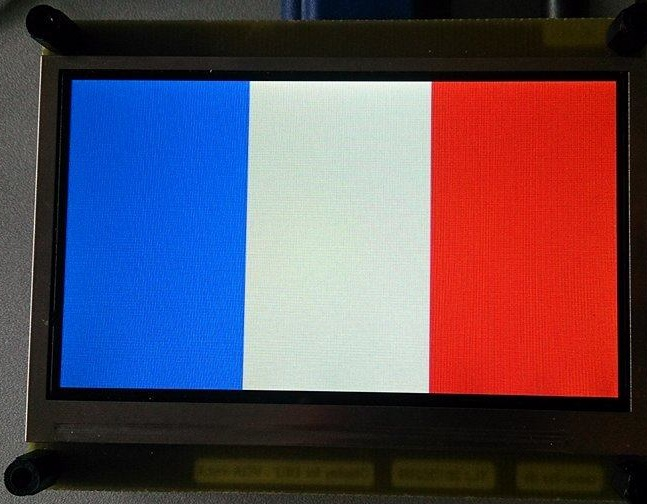
\includegraphics[scale=0.4]{pictures/Oevelse8/opg2/franskFlag}
		\caption{Det franske flag vist på VGA-skærmen}
		\label{fig:frenchFlag}
	\end{figure}

Ved reverse-engineering, gennemgåes templaten som er udleveret, for at opnå en forståelse af dennes funktionalitet.
	
Først i arkitekturen sættes de faste grænser, som VGA-displayet må skrive i, som det ses i kode \ref{lst:Template_Boundaries} nedenfor:
	\begin{lstlisting}[caption={Template Boundaries},label={lst:Template_Boundaries}]
-- horizontal Timing constants for 640 x 480 @ 60Hz
constant hFrontPorch : natural := 16; -- units are number of 25 MHz clocks
constant hBackPorch : natural := 48; 
constant hDataLen : natural := 640;
constant hSynWidth : natural := 96;

-- vertical Timing constants for 640 x 480 @ 60Hz 
constant vFrontPorch : natural := 10;  -- units are number of lines
constant vBackPorch : natural := 33;
constant vDataLen : natural := 480;
constant vSynWidth : natural := 2;

	\end{lstlisting}
	
Herpå oprettes signaler for de countere og flag som benyttes, for at holde styr på områderne der skal skrives i, af programmet, som det ses i kode \ref{lst:Counters}:
\begin{lstlisting}[caption={Signal declaration},label={lst:Counters}]
-- signal declaration
signal hSyncCounter, vSyncCounter : integer range 0 to 1023; -- contrain integer to 10 bit.
signal hSyncOut,vSyncOut,clk25,vBlank,hBlank : std_logic;
\end{lstlisting}
	
Herpå halveres de 50 MHz til 25 MHZ allerførst i processen og vores egen procedure benyttes, trigget af forskellige clocks (hhv 25MHz signalet og hSyncOut).

Sidst findes koden for område-begrænsingen, der sætter farverne for diverse afgrænsede områder af flaget. Disse bliver bestemt ved farvekoderne inden for rød, grøn og blå.

\newpage
\item[2)]

Vi har fulgt underpunkterne i øvelses-vejledning og skrevet proceduren for \textit{\textbf{syncGenerator}} som det kan ses i figur \ref{lst:Procedure_code}:
\begin{lstlisting}[caption={syncGenerator Procedure Code},label={lst:Procedure_code}]

BLABLABLA, SE MIN KODE, DEN ER LANG SOM X10. ALT HVAD JEG EJER, DET ER LANGT SOM DEN. DET ER FORDI AT CECIL HUN ER FRANSKMAND, OG FORDI AT LASSE ER MIN VEN.

	\end{lstlisting}

\item[3)] 

Vi har downloadet programmet til DE2-boardet og opnår flaget som ses på figur \ref{fig:frenchFlag}.
\end{enumerate}